\documentclass{ctexart}
\usepackage{listings}
\usepackage{ctex}
\usepackage{geometry}
\usepackage{graphicx}
\usepackage{float}
\usepackage[colorlinks=true,linkcolor=black]{hyperref}
\usepackage[format=hang,font=small,textfont=it]{caption}
\usepackage[nottoc]{tocbibind}
\usepackage{fontspec}
\usepackage{xeCJK}
\setCJKmainfont{楷体}
\geometry{a4paper,centering,scale=0.8}

\begin{document}
\begin{titlepage}
    \begin{center}
    \phantom{Start!}
	\vspace{3cm}
       \center{\zihao{1} 计算机网络课程设计}
        {
        \setlength{\baselineskip}{40pt}
        \vspace{1cm}
        \zihao{-2}
        \center{DNS中继服务器实验报告}
        \vspace{3.5cm}
        \center{
            \begin{tabular}{cc}
            班\qquad 级:& \underline{~~~~~~2014211306~~~~~~}  \\
        	学\qquad 号:& \underline{~~~~~~2014211281~~~~~~}  \\
        	姓\qquad 名:& \underline{~~~~~~~~黄智伟~~~~~~~~~}  \\
        	教\qquad 师:& \underline{~~~~~~~~高占春~~~~~~~~~}  \\
        	% 实验时间:& \underline{ ~~~~~~2017.5.25~~~~~~~ }  \\
        	\end{tabular}
        }
        \vspace{5cm}
        \center{2017.5.25}
        }
    \end{center}
\end{titlepage}

\pagebreak[4]

\tableofcontents

\pagebreak[4]

\section{系统的功能设计}
\label{sec:purpose}
设计一个DNS服务器程序,DNS中继服务器读入“IP地址-域名”对照表,并以此响应客户端的DNS请求。当
客户端查询域名对应的IP地址时,用域名检索该对照表,产生三种可能检索结果:
\begin{enumerate}
    \item 当检索到的IP地址为0.0.0.0,回复“域名不存在”的报错消息,实现不良网站拦截的功能;
    \item 当检索为普通IP地址,则向客户端返回该地址,实现服务器功能;
    \item 当表中未检到该域名,则向因特网DNS服务器发出查询,并将结果返给客户端,实现中继功能。
\end{enumerate}
\ \ \ \ \ \ 考虑多个计算机上的客户端会同时查询,需要进行消息ID的转换。同时DNS中继服务器还
实现了可以指定远程DNS服务器IP地址,指定“IP地址-域名”对照表的文件位置以及多种级别的调试信息
的输出。

\section{模块划分}
\label{sec:module}
\begin{enumerate}
    \item 读取文件模块:从用户指定的路径读入“IP地址-域名”对照表
    \item 运行模块:接收客户端请求,并放入线程池中运行
    \item 处理请求模块:解析请求,并进行相应的处理
    \item 构建数据包模块:按照RFC1035协议构造出相应回复的数据包
    \item 转发模块:进行ID转换,转发客户端请求给远端DNS服务器,接受远程客户端的回复并转发给客户端
\end{enumerate}
\begin{figure}[H]
  \centering
  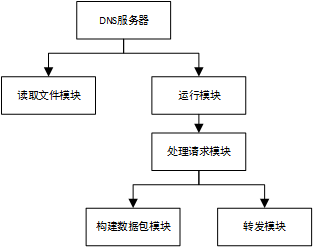
\includegraphics[width=15cm,height=10cm]{img/module.png}
  \caption{模块调用图}
\end{figure}

\section{软件流程图}
\label{sec:chart}
\begin{figure}[H]
  \centering
  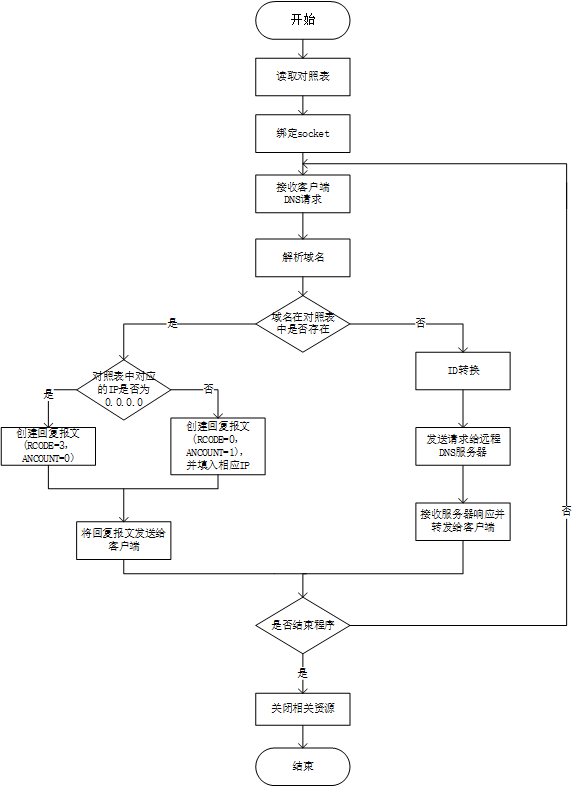
\includegraphics[width=15cm]{img/chart.png}
  \caption{软件流程图}
\end{figure}

\section{测试用例以及运行结果}
\label{run_result}
1.命令行提示:
\begin{figure}[H]
  \centering
  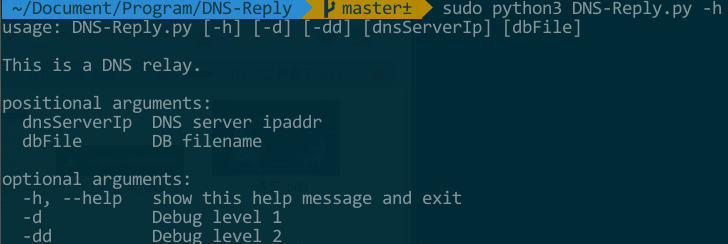
\includegraphics[width=15cm]{img/help.png}
\end{figure}

2.使用默认参数:
\begin{figure}[H]
  \centering
  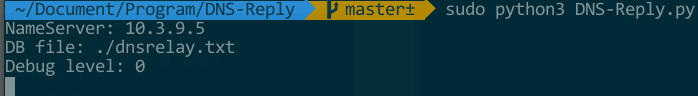
\includegraphics[width=15cm]{img/default.png}
\end{figure}

\ \ \ \ 运行结果:
\begin{figure}[H]
  \centering
  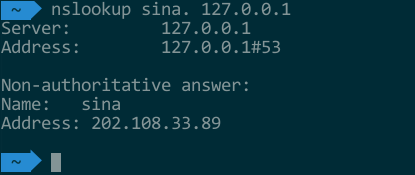
\includegraphics[width=15cm]{img/default-result.png}
\end{figure}

3.调试级别1,指定远程DNS服务器地址,指定对照表文件位置:
\begin{figure}[H]
  \centering
  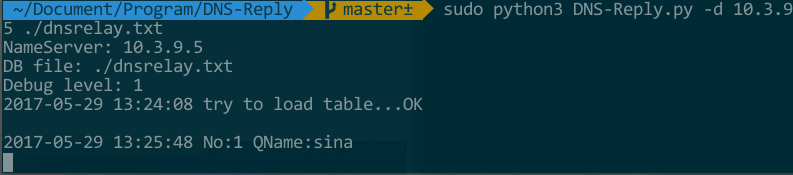
\includegraphics[width=15cm]{img/debug-level-1.png}
\end{figure}

\pagebreak[4]

\ \ \ \ 运行结果:
\begin{figure}[H]
  \centering
  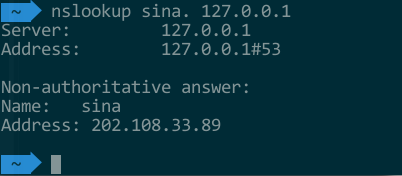
\includegraphics[width=15cm]{img/debug-level-1-result.png}
\end{figure}

4.调试级别2,指定远程DNS服务器地址,指定对照表文件位置:
\begin{figure}[H]
  \centering
  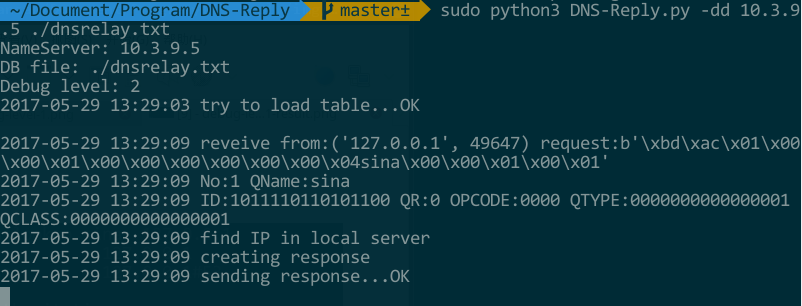
\includegraphics[width=15cm]{img/debug-level-2.png}
\end{figure}

\ \ \ \ 运行结果(查找对照表里存在且不为"0.0.0.0"的域名,即服务器功能):
\begin{figure}[H]
  \centering
  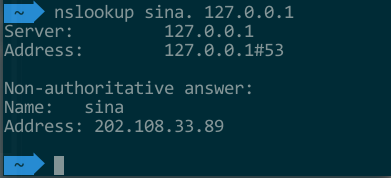
\includegraphics[width=15cm]{img/debug-level-2-local-result.png}
\end{figure}

\pagebreak[4]

\ \ \ \ 运行结果(查找对照表里存在且为"0.0.0.0"的域名,即不良网站拦截功能):
\begin{figure}[H]
  \centering
  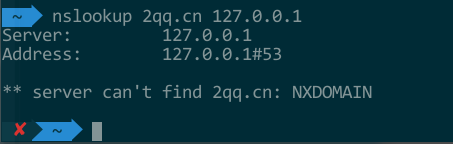
\includegraphics[width=15cm]{img/debug-level-2-local-0-result.png}
  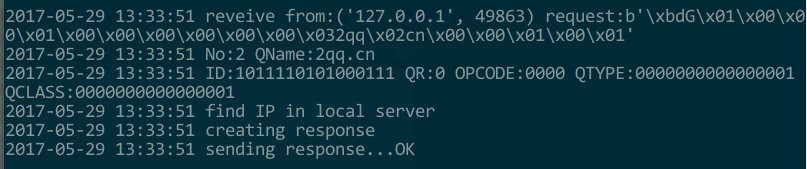
\includegraphics[width=15cm]{img/debug-level-2-local.png}
\end{figure}

\ \ \ \ 运行结果(查找对照表里不存在的域名,即中继功能):
\begin{figure}[H]
  \centering
  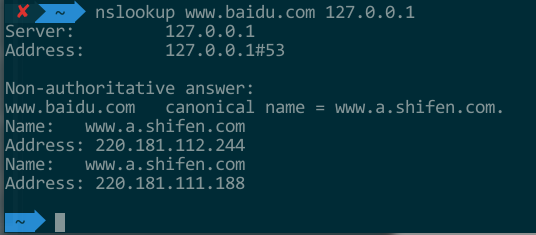
\includegraphics[width=15cm]{img/debug-level-2-remote-result.png}
  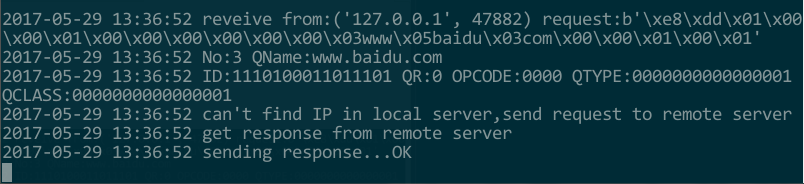
\includegraphics[width=15cm]{img/debug-level-2-remote.png}
\end{figure}

\pagebreak[4]

\section{调试中遇到并解决的问题}
\label{question}
\begin{enumerate}
    \item 问题:刚开始发现域名字段是不定长,不会解析域名字段\\
          解决:查阅资料后发现域名是先用数字表明分段的字符个数,再接着字符(省略小数点'.'),
          字符个数为0时域名字段才结束,之后开始编码解析域名字段
    \item 问题:查询对照表中存在且不为"0.0.0.0"的域名时,返回的IP地址与对照表中相应域名对应
          的IP不一致\\
          解决:查阅资料得,网络字节流是大端序,与Intel x86字节流的小端序正好相反,故错误.
          之后修改代码,问题解决
    \item 问题:由于使用了多线程,访问和修改一些线程间的共享资源存在问题,导致出现错误\\
          解决:采用线程锁,解决线程间共享资源的访问与修改
    \item 问题:由于使用了多线程,同时处理多个客户端请求,当多个客户端请求均为对照表中不存在的
          域名时,向远程DNS服务器转发存在ID一致的问题\\
          解决:进行ID转换,转换规则为:若存在与自己ID一直的请求,则ID加1
    \item 问题:当客户端查询对照表中不存在的域名时,程序向远程DNS服务器转发,有时远程DNS服务器
          响应时间过长,导致线程阻塞\\
          解决:使用定时器,设置远程服务器3.5秒未响应,则停止等待,释放资源,且不回复客户端,
          使客户端超时重发
\end{enumerate}

\section{课程设计工作总结}
\label{summary}
    此次课程设计为实现一个DNS中继服务器。具有不良网站拦截功能,DNS服务器功能及中继功能这三个
基本功能,同时具有指定远程DNS服务器IP地址及本地"IP-域名"对照表文件位置的功能。\\

    由于此次课程设计依赖于RFC 1035协议,所以在进行实际编码实现之前,我首先阅读了RFC 1035
文档.由于文档是英文编写的,刚开始学习时,遇到了很多问题.但是在询问老师及同学之后,对文档
有了一定的了解,之后开始编码实现.\\

    此次的课程设计,使用到了socket编程以及wireshark等抓包软件,我也从中学到了很多.通过此次
课程设计,我掌握了一定的socket编程知识,也对DNS数据报的格式有了一定的了解,同时也明白了DNS
服务器的工作原理及流程.\\

    在编程实现过程中,由于使用了多线程,因此进行了ID转换,同时也对线程间的共享资源进行了加锁操作,
以便共享资源能正确的被访问.虽然在这期间遇到了很多问题,但是也让我更加了解了多线程编程以及锁机制,.
同时为了防止线程阻塞,对socket进行了定时操作,超过一定时间未回复,则放弃等待,释放资源,处理下一
请求.这是为了服务器的性能做出的考虑,这也让我明白了有时候为了性能,不得不放弃一些服务质量.

\end{document}
